\section{Application to a Domain Decomposition Method}
\label{sec:DDM}

\indent The discrete approximations \eqref{eq:appDiscTBCP0} for the Transparent Boundary Conditions for the equation \eqref{eq:DKdV} will be applied as Interface Boundary Conditions (IBC) in a Domain Decomposition Method (DDM). Firstly, following \cite{Japhet2003}, we will briefly describe the DDM that we will consider here, and after we will describe and test the incorporation of the proposed IBCs.

\subsection{The Schwarz Method}

\indent Domain Decomposition Methods allow to decompose a domain $\Omega$ in multiple subdomains $\Omega_i$ (that can possibly overlap) and solve the problem in each one of them. Therefore, one must find functions that satisfies the PDE in each subdomain and that match on the interfaces. 

\indent The first DDM developed was the Schwarz method, which consists on an iterative method : in the case of a evolution problem, the solution  $u_i^{n,\infty}$, in each time step $t_n$ and each subdomain $\Omega_i$, is computed as the convergence of the solution obtained in each iteration, $u_i^{n,k}, \ \ k\geq 0$. 

\indent We will consider here the additive Schwarz method (ASM), in which the Interface Boundary Conditions are always constructed using the solution $u_j^{n,k-1}, \ \ j \neq i$ of the previous iteration in the neighbor subdomains. Therefore, in each interface between the subdomains $\Omega_i$ and $\Omega_j$, the boundary condition for the problem in $\Omega_i$ is

$$\mathcal{B}_i(u_i^{n,k+1}) = \mathcal{B}_i(u_j^{n,k})$$

\noindent where $\mathcal{B}_i$ denotes the operator of the IBC.

\indent Without loss of generality, in the following we will consider a domain $\Omega$ decomposed in two non-overlapping subdomains, $\Omega_1$ and $\Omega_2$, with $\Gamma = \Omega_1 \bigcap \Omega_2$.

\indent When implementing a Schwarz methods, one must define appropriate operators $\mathcal{B}_i$ such that :

\begin{itemize}
\item The solution $u_i$ in each subdomain $\Omega_i$ converges to $u|_{\Omega_i}$, i.e, the solution $u$, restricted to $\Omega_i$, of the problem in the monodomain $\Omega$;
\item The method shows a fast convergence.
\end{itemize} 

\indent In fact, accordingly to \cite{Japhet2003}, the optimal additive Schwarz method for solving the problem 

\begin{equation*}
\begin{cases}
\mathcal{A}(u) = f \ \ \text{in} \ \ \Omega\\
u = 0 \ \ \text{on} \ \ \partial\Omega\\
\end{cases}
\end{equation*}

\noindent where $\mathcal{A}$ is a partial differential operator, is the one which uses as Interface Boundary Conditions the exact Transparent Boundary Conditions, given by

$$B_i(u) = \frac{\partial}{\partial n_i}u + D2N(u)$$

\noindent where $\partial n_i$ is the outward normal to $\Omega_i$ on $\Gamma$ , and the D2N (Dirichlet to Neumann) operator is defined by

$$\left. D2N : \alpha(x) \mapsto \frac{\partial}{\partial n_i^c}v \right\rvert_\Gamma$$

\noindent with $\alpha$ defined on $\Gamma$. $v$ is solution of the following problem, solved in the complementary set of $\Omega_i$, denoted by $\Omega_i^c$

\begin{equation*}
\begin{cases}
\mathcal{A}(v) = f \ \ \text{in} \ \ \Omega_i^c\\
v = 0 \ \ \text{on} \ \ \partial \Omega_i \backslash \Gamma \\
v = \alpha \ \ \text{on} \ \ \Gamma
\end{cases}
\end{equation*}

\indent The ASM using such exact TBCs is optimal in the sense that it converges in two iterations, and no other ASM can converge faster. Nevertheless, these TBC, in general, are not simple to compute both analtically and numerically. More specifically, they are nonlocal in time, so they must be approximated for an efficient numerical implementation \cite{Xavieretal2008}. It is in this context that we propose the implementation of our approximate TBCs as Interface Boundary Conditions for the ASM.

\subsection{ASM with the approximate TBCs for the dispersion equation}

\indent The resolution of the dispersion equation \eqref{eq:DKdV} with the Additive Schwarz method, using the constant polynomial approximation for the TBCs, is written as

\begin{equation}
    \label{eq:problemDDM1}
    \begin{cases}
        (u_1^{n,k+1})_t + (u_1^{n,k+1})_{xxx} = 0 , \ \ x \in \Omega_1, \ \ t \geq t_0\\
        u_1^{n,0} = u_1^{n-1,\infty} , \ \ x \in \Omega_1 \\
        \Upsilon_1^{c_L}(u_1^{n+1,k+1},-L) = 0, \\ 
        \Theta_2^{c_R}(u_1^{n+1,k+1},0) = \Theta_2^{c_R}(u_2^{n,k},0) , \\
        \Theta_3^{c_R}(u_1^{n+1,k+1},0) = \Theta_3^{c_R}(u_2^{n,k},0)
     \end{cases}
\end{equation}

\begin{equation}
    \label{eq:problemDDM2}
    \begin{cases}
        (u_2^{n,k+1})_t + (u_2^{n,k+1})_{xxx} = 0 , \ \ x \in \Omega_2, \ \ t \geq t_0\\
        u_2^{n,0} = u_2^{n-1,\infty} , \ \ x \in \Omega_2 \\
        \Theta_1^{c_L}(u_2^{n+1,k+1},0) = \Theta_1^{c_L}(u_1^{n,k},0) \\
        \Upsilon_2^{c_R}(u_2^{n+1,k+1},L) = 0 \\
        \Upsilon_3^{c_R}(u_2^{n+1,k+1},L) = 0
     \end{cases}
\end{equation}

\noindent where $ \Upsilon_i, \ \ i=1,2,3$, are the external boundary conditions (i.e, defined on $\partial \Omega_i \backslash \Gamma$).

\indent Considering that we want to analyze and minimize the error due to the application of a Domain Decomposition Method, the reference solution $u^{ref}$ in our study will be the solution of the monodomain problem

\begin{equation}
	\label{eq:problemMonodomain}
	\begin{cases}
	u_t + u_{xxx} = 0, \ \ x \in \Omega, \ \ t \in [t_0, t_0+\Delta t] \\
	u(t_0,x) = u^{exact}(t_0,x) , \ \ x \in \Omega \\ 
	\Upsilon_1(u,-L) = 0, \ \ t \in [t_0, t_0+\Delta t] \\
	\Upsilon_2(u,L) = 0, \ \ t \in [t_0, t_0+\Delta t] \\
	\Upsilon_3(u,L) = 0, \ \ t \in [t_0, t_0+\Delta t]
	\end{cases}
\end{equation}
	
\indent We notice that we will always compare the solutions computed along only one time step. This is necessary for the separated study of the DDM method (without influence, for example, of the error accumulated along the time steps, due to the temporal discretization).

\indent The external BCs $ \Upsilon_i, \ \ i=1,2,3$ are independent of the interface BCs. Here, we will consider $\Upsilon_1 = \Theta_1^{c_L = 1.0}$, $\Upsilon_2 = \Theta_2^{c_R = 0.0}$ and $\Upsilon_3 = \Theta_3^{c_R = 0.0}$, which gives

\begin{equation}
	\label{eq:externalBCsDDM}
	\begin{gathered}
	\Upsilon_1(u,x) = u - u_x + u_{xx} = 0\\
	\Upsilon_2(u,x) = u = 0\\
	\Upsilon_3(u,x) = u_x = 0\\
	\end{gathered}
\end{equation}

\indent This choice was made based on the easy implementation and the good results provided by the coefficients $c_L = 1.0$ and $c_R = 0.0$ in approximating the analytical solution in $\Omega$ (as shown in the table \ref{tab:firstTestsP0}). Nevertheless, it does not have much importance in the study that we will done here, as we want to study exclusively the behavior of the DDM. The only restriction for an appropriate study is that the external BCs for computing $u_{ref}$ must be the same $\Upsilon_i, \ \ i=1,2,3$, used for each subdomain in the DDM, as we done in \eqref{eq:problemDDM1}-\eqref{eq:problemDDM2} and \eqref{eq:problemMonodomain}.

\paragraph{Remarks on the notation}

%\indent From here to the end of this paper, we will focus exclusively on the error produced by the DDM, compared to the referential solution, independently of the other possible components of the error compared to the analytical solution (external boundary conditions, error accumulation over the time steps, for example, as discussed in the introduction. 

\indent As the following study will be made considering the execution of the method over only one time step, we can suppress the index denoting the instant $t_n$ and use a clearer notation for the solution : $u_j^i$, where $i$ indicates the subdomain $\Omega_i$ (or, in the case of the reference solution, $i = ref$, and in the convergence of the method, $i = *$) and $j$ indicates the spatial discrete position. In the cases where the iterative process is taken into account, we will add the superscript $k$ to indicate the iteration.

\indent Concerning the spatial discretization, the monodomain $\Omega$ will be divided in $2N + 1$ homogeneously distributed points, numbered from $0$ to $2N$. In all the analytical description, we will consider that the two subdomains $\Omega_1$ and $\Omega_2$ have the same number of points, respectively $x_0,...,x_N$ and $x_N,...,x_{2N}$. The interface point $x_N$ is common to the two domains, having different computed solutions $u_N^1$ and $u_N^2$ in each one of them. Evidently, we expect, at the convergence of the ASM, that $u_N^1 = u_N^2 = u_N^*$

\subsection{Discretization of the problem}

\indent For the interior points of each one of the domains, we will consider a second order spatial discretization of the equation (\ref{eq:DKdV}).

\begin{equation}
    \label{eq:FDdiscretization}
    \frac{u_j^i - \alpha_j^i}{\Delta t} + \frac{-\frac{1}{2}u_{j-2}^i + u_{j-1}^i - u_{j+1}^i + \frac{1}{2}u_{j+2}^i }{\Delta x ^3} = 0
\end{equation}

\noindent which is valid for $j=2,...,N-2$ in the case $i=1$; for $j=N+2,...,2N-2$ in the case $i=2$; and for $j=2,...,2N-2$ in the case $i=ref$. In the above expression, $\alpha_j^i$ is a given data (for example, the converged solution in the previous time step).

\indent For the points near the boundaries, we use second order uncentered discretizations or an appoximate TBC. Considering that one TBC is written for the left boundary and two for the right one, we have to impose an uncentered discretization only for the second leftmost point of the domain. For example, for the point $x_1$ : 

\begin{equation}
    \label{eq:uncenteredFDdiscretization0}
    \frac{u_{1}^2 - \alpha_{1}^2}{\Delta t} + \frac{-\frac{5}{2}u_{1}^2 + 9u_{2}^2 - 12 u_{3}^2 + 7\frac{1}{2}u_{4}^2 -\frac{3}{2}u_{5}^2}{\Delta x ^3} = 0
\end{equation}

\noindent and similarly to the other points near the boundaries.

\indent In the resolution of the problem in $\Omega_1$, two interface boundary conditions are imposed (corresponding to $\Theta_2$ and $\Theta_3$) to the discrete equations for the points $x_{N-1}$ and $x_N$. On the other hand, in the resolution of the problem in $\Omega_2$, only one interface boundary condition is used (corresponding to $\Theta_1$), being imposed to the point $x_N$.

\paragraph{Remark : modification of the reference solution}

\indent  Even if the DDM with the proposed Interface Boundary Conditions is compatible with the monodomain problem (which we will see that is not the case), the solution of the DDM does not converge exactly to $u^{ref}$, for a reason that does not depend on the expression of the IBCs, but on the fact that for each domain we write two IBCs in the left boundary and only one on the right. We are using a second order centered discretization for the third spatial derivative (which uses a stencil of two points in each side of the central point), implying that we must write an uncentered discretization for the point $x_{N+1}$ when solving the problem in $\Omega_2$. Therefore, this point does not satisfy the same discrete equation as in the reference problem. In order to avoid this incompatibility and allow us to study the behavior of the DDM, we will modify the discretization for the point $u_{N+1}$ in the monodomain problem, using the same second-order uncentered expression :

\begin{equation*}
    \label{eq:uncenteredFDdiscretizationN}
    \frac{u_{N+1}^2 - \alpha_{N+1}^2}{\Delta t} + \frac{-\frac{5}{2}u_{N+1}^2 + 9u_{N+2}^2 - 12 u_{N+3}^2 + 7\frac{1}{2}u_{N+4}^2 -\frac{3}{2}u_{N+1}^2}{\Delta x ^3} = 0
\end{equation*}

\indent The figure \ref{fig:discretizations} resumes the discretizations imposed to each point in the monodomain and the DDM problems, as described above:

\indent 

\begingroup
\tikzstyle{label} =[above,font=\tiny]
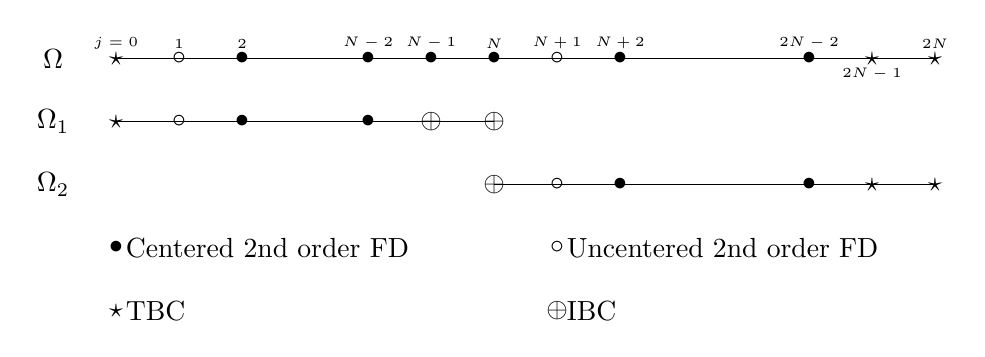
\begin{tikzpicture}[scale = .8]
	\coordinate (Alabel) at (-1,3);
	\coordinate (Aa) at (0,3);
	\coordinate (Ab) at (1,3);
	\coordinate (Ac) at (2,3);
	\coordinate (Ad) at (4,3);	
	\coordinate (Ae) at (5,3);	
	\coordinate (Af) at (6,3);	
	\coordinate (Ag) at (7,3);	
	\coordinate (Ah) at (8,3);	
	\coordinate (Ai) at (11,3);
	\coordinate (Aj) at (12,3);
	\coordinate (Ak) at (13,3);
	
	\draw (Aa) -- (Ak);
	\draw (Alabel) node {$\Omega$}; 
	\draw (Aa) node[label] {$j=0$};
	\draw (Ab) node[label] {$1$};
	\draw (Ac) node[label] {$2$};
	\draw (Ad) node[label] {$N-2$};
	\draw (Ae) node[label] {$N-1$};
	\draw (Af) node[label] {$N$};
	\draw (Ag) node[label] {$N+1$};
	\draw (Ah) node[label] {$N+2$};
	\draw (Ai) node[label] {$2N-2$};
	\draw (Aj) node[below,font=\tiny] {$2N-1$};
	\draw (Ak) node[label] {$2N$};
		
	\draw (Aa) node {$\star$};
	\draw (Ab) node {$\circ$};
	\draw (Aj) node {$\star$};
	\draw (Ak) node {$\star$};
	
	\draw (Ac) node{$\bullet$};
	\draw (Ad) node {$\bullet$};
	\draw (Ae) node {$\bullet$};
	\draw (Af) node{$\bullet$};	
	\draw (Ag) node{$\circ$};
	\draw (Ah) node {$\bullet$};
	\draw (Ai) node {$\bullet$};


	\coordinate (Blabel) at (-1,2);	
	\coordinate (Ba) at (0,2);
	\coordinate (Bb) at (1,2);
	\coordinate (Bc) at (2,2);
	\coordinate (Bd) at (4,2);	
	\coordinate (Be) at (5,2);	
	\coordinate (Bf) at (6,2);	

	\draw (Ba) -- (Bf); 
	
	\draw (Blabel) node {$\Omega_1$}; 
	\draw (Ba) node {$\star$};
	\draw (Bb) node {$\circ$};
	
	\draw (Bc) node {$\bullet$};
	\draw (Bd) node {$\bullet$};
	
	\draw (Be) node {$\oplus$};
	\draw (Bf) node {$\oplus$};	
	
	\coordinate (Clabel) at (-1,1);	
	\coordinate (Cf) at (6,1);	
	\coordinate (Cg) at (7,1);	
	\coordinate (Ch) at (8,1);	
	\coordinate (Ci) at (11,1);
	\coordinate (Cj) at (12,1);
	\coordinate (Ck) at (13,1);
		
	\draw (Cf) -- (Ck); 
	\draw (Clabel) node {$\Omega_2$}; 
	\draw (Cf) node{$\oplus$};
	\draw (Cg) node{$\circ$};
	\draw (Ch) node{$\bullet$};	
	\draw (Ci) node{$\bullet$};	
	\draw (Cj) node {$\star$};
	\draw (Ck) node{$\star$};
	
	%% Legend
	\draw (0,0) node {$\bullet$} node[right] {Centered 2nd order FD};
	\draw (7,0) node {$\circ$} node[right] {Uncentered 2nd order FD};
	\draw (0,-1) node {$\star$} node[right] {TBC};
    \draw (7,-1) node {$\oplus$} node[right] {IBC};
	
\end{tikzpicture}
\captionof{figure}{Scheme indicating the discretization imposed to each point in the monodomain and the DDM problems \label{fig:discretizations}}
\endgroup


\subsection{Corrections for the approximate IBCs}

\indent When using approximate TBCs in the ASM, one should guarantee that the converged solutions $u^*$ satisfy the same equation as the solution $u_{ref}$ of the monodomain problem. Nevertheless, \begingroup \color{red}{usually this property is not verified by DDMs} \endgroup, which is the case of the method proposed here : one can easily see that, in the convergence, the solution $u^*$ does not satisfy the discrete equation \eqref{eq:FDdiscretization} on the points where the IBCs are imposed (the poins $x_{N-1},x_N \in \Omega_1$ and $x_N \in \Omega_2$).

\indent Therefore, we will formulate modified TBCs for the ASM in order to avoid this problem  :

\begin{equation}
	\label{eq:correctedTBC}
    \begin{gathered}
        \Theta_1^{c_L}(u_2^{n+1,k+1}) + \theta_1 = \Theta_1^{c_L}(u_1^{n,k}) + \theta_1' \\
        \Theta_2^{c_R}(u_1^{n+1,k+1}) + \theta_2 = \Theta_2^{c_R}(u_2^{n,k}) + \theta_2' \\
        \Theta_3^{c_R}(u_1^{n+1,k+1}) + \theta_3 = \Theta_3^{c_R}(u_2^{n,k}) + \theta_3'
    \end{gathered}
\end{equation}

\noindent with $\theta_i, \theta_i'$ given by

\begin{gather*}
    \theta_1 = \Delta x c_L \frac{u_{N+1}^2 - 2u_{N}^2 + u_{N-1}^1}{\Delta x^2} + c_L^2\frac{\Delta x}{\Delta t} \left( u_{N}^2 - \alpha_{N}^2 \right)\\
    \theta_1' = - c_L^2\frac{\Delta x}{\Delta t} \left( u_{N}^1 - \alpha_{N}^1 \right)
\end{gather*}

\begin{equation*}
\begin{gathered}
    \theta_2 = \frac{\Delta x}{\Delta t} c_R^2 (u_N^1 - \alpha_N^1) \\
    \theta_2' = -\frac{\Delta x}{\Delta t} c_R^2 (u_N^2 - \alpha_N^2)
\end{gathered}
\end{equation*}

\begin{equation*}
\begin{gathered}
    \theta_3 = 2\frac{\Delta x}{\Delta t} \left[-\Delta x(u_{N-1}^1 - \alpha_{N-1}^1) - c_R (u_N^1 - \alpha_N^1) \right] + \Delta x \frac{u_{N-3}^1 - 2u_{N-2}^1 + u_{N-1}^1}{\Delta x^2} \\
    \theta_3' = 0
\end{gathered}
\end{equation*}

\indent It is straightforward to verify that the DDM problem with these modifications in the TBCs assure that the converged solution $u^*$ satisfies, in every point, the same discrete equations as the solution $u^{ref}$ of the monodomain problem \eqref{eq:problemMonodomain}.

\indent We notice that all the modification terms $\theta_i,\theta_i', \ i = 1,2,3$ are of order $O(\Delta x)$ (they are composed of discrete versions of time derivatives and second spatial derivatives multiplied by $\Delta x$). It is essential to assure that these terms are small, in order not to cause substantial modifications to the respective approximate TBCs $\Theta_i$.


\subsection{Optimization of the IBCs (speed of convergence)}

\indent Our objective now is to optimize the IBCs in the sense of minimizing the number of iterations of the ASM until the convergence. We will make a very large set of tests in order to find the coefficients $c_L$ and $c_R$ (i.e., the constant polynomial approximation for the TBC) that provides the fastest convergence. In a first moment, we will make this study with fixed time step and space step, in order to analyze exclusively the influence of the coefficient, and after we will introduce these two parameters into the study.

\indent As we are interested in the speed with which the solution of the DDM method converges to the reference solution, the criteria of convergence used is

\begin{equation*}
\label{eq:criteriaConvergence}
	e^{\Omega,k} \leq \epsilon
\end{equation*}

\noindent with $\epsilon = 10^{-9}$ and 

\begin{equation*}
	e^{\Omega,k} = ||u^{ref}_N - u^{k}_N||_2 = \sqrt{\Delta x \left[ \sum_{j=0}^N{(u^{ref}_j - u^{1,k}_j)^2 } + \sum_{j=N}^{2N}{(u^{ref}_j - u^{2,k}_j)^2 } \right] }
\end{equation*}
 
\indent In order to simplify the tests and avoid too expensive computations, we will always consider $c_L = c_R = c$ in this optimization. The range of tested coefficients is $[-10.0, 20.0]$ (chosen after initial tests to identify a proper interval), with a step equal to  $0.1$ between them (or even smaller, up to $0.005$, in the regions near the optimal coefficients), and the maximal number of iterations is set to 100.

\subsubsection{Test varying the initial time step and the interface position}

\indent As said above, in the first set of tests we will consider a fixed time step $\Delta t = 20/2560 = 0.0078125$ and a fixed mesh size $\Delta x = 12/500 = 0.024$. Moreover, we will consider two subsets of tests, that will allow us to study the speed of convergence with different initial conditions and different sizes of the subdomains:

\begin{enumerate}
	\item Tests varying the initial time step $t_0$, with the interface in the center of the monodomain $\Omega = [-6,6]$;
	\item Tests varying the position of the interface ($x_{interface} = -L + \alpha 2L$, where $L = 6$ and $0 < \alpha < 1$), for a fixed initial time $t_0 = 0.78125$.
\end{enumerate}

\indent In all the cases, the reference solution $u^{ref}$ will be the solution of the monodomain problem \eqref{eq:problemMonodomain}.

\indent The results are summarized in the figures \ref{fig:optimVarT0} and \ref{fig:optimVarInterface}, with the number of iterations plotted as function of the coefficient $c$. For the sake of clearness, the results for negative and positive coefficients are shown in separated graphs. They show a very similar behavior of all the curves, with two minimums for $c < 0$ and other two for $c>0$, which have practically the same value for all the curves (approximately -1.35, -0.10, 0.20 and 4.50). The minima closest to zero are associate to a very discontinuous peak, while the other two are associated with smoother curves. A detail of the curves around each minima are shown in the figures \ref{fig:optimVarT0NDetail} to \ref{fig:optimVarT0PDetail2} and \ref{fig:optimVarInterfaceNDetail} to ref{fig:optimVarInterfacePDetail2}. For some curves, the minimum is associated with the coefficients closest to zero, and, for other ones, to the other minimum, but the minimal number of iterations are very similar (between 5 and 7).

\begingroup
\begin{minipage}{.5\linewidth}
\begin{center}
	\includegraphics[scale=.4]{figures/FinalFigures/NiterxCoefVarT0FinalVersionN.png}
	\captionof{subfigure}{General view for negative coefficients}
\end{center}
\end{minipage}
\begin{minipage}{.5\linewidth}
\begin{center}
	\includegraphics[scale=.4]{figures/FinalFigures/NiterxCoefVarT0FinalVersionP.png}
	\captionof{subfigure}{General view for positive  coefficients}
\end{center}
\end{minipage}
\begin{minipage}{.5\linewidth}
\begin{center}
	\includegraphics[scale=.4]{figures/FinalFigures/NiterxCoefVarT0FinalVersionNDetail.png}
	\captionof{subfigure}{Detail around one of the optimal negative coefficients  \label{fig:optimVarT0NDetail}}
\end{center}
\end{minipage}
\begin{minipage}{.5\linewidth}
\begin{center}
	\includegraphics[scale=.4]{figures/FinalFigures/NiterxCoefVarT0FinalVersionNDetail2.png}
	\captionof{subfigure}{Detail around the other optimal negative coefficient  \label{fig:optimVarT0NDetail2}}
\end{center}
\end{minipage}
\begin{minipage}{.5\linewidth}
\begin{center}
	\includegraphics[scale=.4]{figures/FinalFigures/NiterxCoefVarT0FinalVersionPDetail.png}
	\captionof{subfigure}{Detail around one of the optimal positive coefficients \label{fig:optimVarT0PDetail} }
\end{center}
\end{minipage}
\begin{minipage}{.5\linewidth}
\begin{center}
	\includegraphics[scale=.4]{figures/FinalFigures/NiterxCoefVarT0FinalVersionPDetail2.png}
	\captionof{subfigure}{Detail around the other optimal positive coefficient  \label{fig:optimVarT0PDetail2}}
\end{center}
\end{minipage}
	\captionof{figure}{Number of iterations until the convergence as function of the coefficient of the TBC (for a fixed interface and different values of $t_0$) \label{fig:optimVarT0}}
\endgroup

\begingroup
\begin{minipage}{.5\linewidth}
\begin{center}
	\includegraphics[scale=.4]{figures/FinalFigures/NiterxCoefVarInterfaceFinalVersionN.png}
	\captionof{subfigure}{General view for negative coefficients}
\end{center}
\end{minipage}
\begin{minipage}{.5\linewidth}
\begin{center}
	\includegraphics[scale=.4]{figures/FinalFigures/NiterxCoefVarinterfaceFinalVersionP.png}
	\captionof{subfigure}{General view for positive coefficients }
\end{center}
\end{minipage}
\begin{minipage}{.5\linewidth}
\begin{center}
	\includegraphics[scale=.4]{figures/FinalFigures/NiterxCoefVarInterfaceFinalVersionNDetail.png}
	\captionof{subfigure}{Detail around one of the optimal negative coefficients  \label{fig:optimVarInterfaceNDetail}}
\end{center}
\end{minipage}
\begin{minipage}{.5\linewidth}
\begin{center}
	\includegraphics[scale=.4]{figures/FinalFigures/NiterxCoefVarInterfaceFinalVersionNDetail2.png}
	\captionof{subfigure}{Detail around the other optimal negative coefficient  \label{fig:optimVarInterfaceNDetail2}}
\end{center}
\end{minipage}
\begin{minipage}{.5\linewidth}
\begin{center}
	\includegraphics[scale=.4]{figures/FinalFigures/NiterxCoefVarInterfaceFinalVersionPDetail.png}
	\captionof{subfigure}{Detail around one of the optimal positive coefficient \label{fig:optimVarInterfacePDetail}  }
\end{center}
\end{minipage}
\begin{minipage}{.5\linewidth}
\begin{center}
	\includegraphics[scale=.4]{figures/FinalFigures/NiterxCoefVarInterfaceFinalVersionPDetail2.png}
	\captionof{subfigure}{Detail around the other optimal positive coefficient  \label{fig:optimVarInterfacePDetail2}}
\end{center}
\end{minipage}
	\captionof{figure}{Number of iterations until the convergence as function of the coefficient of the TBC (for a fixed $t_0$ and different positions of the interface) \label{fig:optimVarInterface}}
\endgroup

\indent The figure \ref{fig:errorEvolution} shows the evolution of the error, as function of the iterations, for the five coefficients $c$ that gave the fastest convergences, for a fixed initial instant and a fixed position position of the interface. For other values of $t_0$ and $\alpha$ this graph is similar, concerning the number of iterations and the fact that the convergence is more regular for the coefficients closest to zero, compared to the other optimal coefficients.

\begingroup
\begin{center}
\includegraphics[scale=.5]{figures/FinalFigures/errorEvolutionFixedT0BFinalVersion.png}
\captionof{figure}{Error evolution with the iterations for the fastest results \label{fig:errorEvolution}}
\end{center}
\endgroup

\subsubsection{Tests varying $\Delta t$ and $\Delta x$}

\indent After verifying that the method behaves similarly for every initial condition (i.e., every $t_0$) and every position of the interface, we will now keep these parameters fixed ($t_0 = 0$ and $\alpha = 0.5$) and make new tests with different values of $\Delta t$ (with fixed $\Delta x = 12/250$) and different values of $\Delta x$ (with fixed $\Delta t = 0.02$).

\indent The number of iterations as functions of the coefficients, for some of the tests, are shown in the figure \ref{fig:niterxCoefVarDt} and \ref{fig:niterxCoefVarDx}. The figure \ref{fig:optimalCoefVarDxDtCorrectN} presents the optimal coefficient for each $\Delta t$ or $\Delta x$. Considering the observation we did before about the similar results (i.e, the number of iterations until the convergence) for the four optimal coefficients, we only took into account, for the construction of this curve, the two minima farther from zero : it was done because, as shown  in the figures \ref{fig:niterxCoefVarDt} and \ref{fig:niterxCoefVarDx}, these minima have a strong dependence on $\Delta t$ or $\Delta x$, and we will seek to study this relation.

\begingroup
\begin{minipage}{.5\linewidth}
\begin{center}
	\includegraphics[scale=.45]{figures/FinalFigures/NiterxCoefVarDtdx250FinalVersionNMarshal.png}
\captionof{subfigure}{Negative coefficients}
\end{center}
\end{minipage}
\begin{minipage}{.5\linewidth}
\begin{center}
	\includegraphics[scale=.45]{figures/FinalFigures/NiterxCoefVarDtdx250FinalVersionPMarshal.png}
\captionof{subfigure}{Positive coefficients}
\end{center}
\end{minipage}
\captionof{figure}{Number of iterations until the convergence as function of the coefficient of the TBC, for a fixed $2N = 250$ and different values of $\Delta t$  \label{fig:niterxCoefVarDt}}

\begin{minipage}{.5\linewidth}
\begin{center}
	\includegraphics[scale=.45]{figures/FinalFigures/NiterxCoefVarDxdt2em2FinalVersionN.png}
\captionof{subfigure}{Negative coefficients}
\end{center}
\end{minipage}
\begin{minipage}{.5\linewidth}
\begin{center}
	\includegraphics[scale=.45]{figures/FinalFigures/NiterxCoefVarDxdt2em2FinalVersionP.png}
\captionof{subfigure}{Positive coefficients}
\end{center}
\end{minipage}
\captionof{figure}{Number of iterations until the convergence as function of the coefficient of the TBC, for a fixed $\Delta t = 0.02$ and different values of $\Delta x$ \label{fig:niterxCoefVarDx}}
\endgroup

\begingroup

\endgroup

%\begingroup
%\begin{center}
%	\includegraphics[scale=.5]{figures/NiterxCoefVarDtdx250CorrectN.png}
%\captionof{figure}{Number of iterations until the convergence as function of the coefficient of the TBC (for a fixed $2N = 250$ and different values of $\Delta t$) \label{fig:niterxCoefVarDt}}
%\end{center}
%\endgroup
%
%\begingroup
%\begin{center}
%	\includegraphics[scale=.5]{figures/NiterxCoefVarDxdt2em2CorrectN.png}
%\captionof{figure}{Number of iterations until the convergence as function of the coefficient of the TBC (for a fixed $\Delta t = 0.02$ and different values of $\Delta x$) \label{fig:niterxCoefVarDx}}
%\end{center}
%\endgroup

\begingroup
\begin{center}
	\includegraphics[scale=.5]{{figures/FinalFigures/OptimalCoefVarDxDtFinalVersionMarshal.png}}
	\captionof{figure}{Optimal coefficients as function of the time step and the space step 	\label{fig:optimalCoefVarDxDtCorrectN}}
\end{center}
\endgroup

\indent The figure \ref{fig:optimalCoefVarDxDtCorrectN} suggests that some kind of regressions could be done in order to obtain a curve of the optimal coefficient in function of $\Delta t$ or $\Delta x$. The shapes of the numerical curves indicate that the optimal $c$ shall be function of $\sqrt{\Delta t}$ and $\frac{1}{\Delta x}$. In fact, as shown in the figures \ref{fig:regressionDt} and \ref{fig:regressionDx}, these models provide very good approximations (specially in the case $c = c(\Delta x)$), both quantitatively (with all the coefficients of determination $R^2$  bigger than 0.99) and qualitatively .

\begingroup
\begin{minipage}{.5\linewidth}
\begin{center}
	\includegraphics[scale=.5]{figures/FinalFigures/regressionDtFinalVersionNMarshal.png}
	\captionof{subfigure}{Regression for negative coefficients}
\end{center}
\end{minipage}
\begin{minipage}{.5\linewidth}
\begin{center}
	\includegraphics[scale=.5]{figures/FinalFigures/regressionDtFinalVersionPMarshal.png}
	\captionof{subfigure}{Regression for positive coefficients}
\end{center}
\end{minipage}
\captionof{figure}{Numerical and regression curve for the optimal coefficient as function of $\Delta t$\label{fig:regressionDt}}

\begin{minipage}{.5\linewidth}
\begin{center}
	\includegraphics[scale=.5]{figures/FinalFigures/regressionDxFinalVersionMarshalN.png}
	\captionof{subfigure}{Regression for negative coefficients}
\end{center}
\end{minipage}
\begin{minipage}{.5\linewidth}
\begin{center}
	\includegraphics[scale=.5]{figures/FinalFigures/regressionDxFinalVersionMarshalP.png}
	\captionof{subfigure}{Regression for positive coefficients}
\end{center}
\end{minipage}
\captionof{figure}{Numerical and regression curve for the optimal coefficient as function of $\Delta t$\label{fig:regressionDx}}
\endgroup

\subsection{Partial conclusion}
 
\indent The results presented in this section show that the Domain Decomposition Method proposed here, consisting in the Additive Schwarz Method with our approximate TBCs, is able to provide a fast convergence toward the solution of the monodomain problem. Furthermore, using the corrected TBCs \eqref{eq:correctedTBC}, this convergence is exact. Therefore, we reached our goals of solving the dispersion equation in a finite domain divided in two subdomains.

\indent Moreover, the results of the optimization tests are very satisfying regarding a more general application of our method. Firstly, for fixed spatial and temporal discretizations, we obtained optimal coefficients for the method independently of the initial solution and the size of the subdomains (i.e., independently of the initial instant and the position of the interface). Secondly, we obtained good regression curves for the optimal coefficient as function of $\Delta t$ or $\Delta x$, which could allow the application of the model, with fast convergence, for tests different from the ones made in this study.












%
%
%\indent For the interior points of each one of the domains, we will consider a second order spatial discretization of the equation (\ref{eq:DKdV}).
%
%\begin{equation}
%    \label{eq:FDdiscretization}
%    \frac{u_j^i - \alpha_j^i}{\Delta t} + \frac{-\frac{1}{2}u_{j-2}^i + u_{j-1}^i - u_{j+1}^i + \frac{1}{2}u_{j+2}^i }{\Delta x ^3} = 0
%\end{equation}
%
%\noindent which is valid for $j=2,...,N-2$ in the case $i=1$; for $j=N+2,...,2N-2$ in the case $i=2$; and for $j=2,...,2N-2$ in the case $i=ref$. In the above expression, $\alpha_j^i$ is a given data (for example, the converged solution in the previous time step).
%
%\indent For the points near the boundaries, we use second order uncentered discretizations or the appropriate TBCs. For example, for the point $x_0$ : 
%
%\begin{equation}
%    \label{eq:uncenteredFDdiscretization0}
%    \frac{u_{0}^2 - \alpha_{0}^2}{\Delta t} + \frac{-\frac{5}{2}u_{0}^2 + 9u_{1}^2 - 12 u_{2}^2 + 7\frac{1}{2}u_{3}^2 -\frac{3}{2}u_{4}^2}{\Delta x ^3} = 0
%\end{equation}
%
%\noindent and similarly to the other points near the boundaries.
%
%\indent In the resolution of the problem in $\Omega_1$, two interface boundary conditions are imposed (corresponding to $\Theta_2$ and $\Theta_3$), so the discrete equations for the points $x_{N-1}$ and $x_N$ are written as
%
%\begin{equation}
%	\begin{aligned}
%    \label{eq:TBCsIterOmega1A}
%    && 				&\Theta_2^{c_R}(u_N^1) = \Theta_2^{c_R}(u_N^2) \implies \\ 
%    && \implies & u_N^1 - c_R^2 \frac{u_N^1 - 2u_{N-1}^1 + u_{N-2}^1}{\Delta x^2} = u_N^2 - c_R^2 \frac{u_N^2 - 2u_{N+1}^2 + u_{N+2}^2}{\Delta x^2} 
%    \end{aligned}
%\end{equation}
%
%\begin{equation}
%	\begin{aligned}
%    \label{eq:TBCsIterOmega1B}
%    && 			   & \Theta_3^{c_R}(u_N^1) = \Theta_3^{c_R}(u_N^2) \implies \\
%    && \implies & \frac{u_N^1 - u_{N-1}^1}{\Delta x} + c_R \frac{u_N^1 - 2u_{N-1}^1 + u_{N-2}^1}{\Delta x^2} = \frac{u_{N+1}^2 - u_{N}^2}{\Delta x} + c_R \frac{u_N^2 - 2u_{N+1}^2 + u_{N+2}^2}{\Delta x^2}
%    \end{aligned}
%\end{equation}
%
%\indent In the resolution of the problem in $\Omega_2$, only one interface boundary condition is used (corresponding to $\Theta_1$) :
%
%\begin{equation}
%	\begin{aligned}
%    \label{eq:TBCsIterOmega2}
%    && 				&\Theta_1^{c_L}(u_N^2) = \Theta_1^{c_L}(u_N^1) \implies \\ 
%    && \implies & u_N^2 - c_L \frac{u_{N+1}^2 - u_{N}^2}{\Delta x} + c_L^2 \frac{u_N^2 - 2u_{N+1}^2 + u_{N+2}^2}{\Delta x^2}  =\\
%    && 				& u_N^1 - c_L \frac{u_{N}^1 - u_{N-1}^1}{\Delta x} + c_L^2 \frac{u_N^1 - 2u_{N-1}^1 + u_{N-2}^1}{\Delta x^2}
%    \end{aligned}
%\end{equation}
%
%\indent In the convergence, the expressions \eqref{eq:TBCsIterOmega1A} to \eqref{eq:TBCsIterOmega2} give respectively
%
%\begin{equation*}
%    \label{eq:TBCsCVOmega1A}
%\begin{aligned}
%    && 			    &u_N^* - c_R^2 \frac{u_N^* - 2u_{N-1}^* + u_{N-2}^*}{\Delta x^2} = u_N^* - c_R^2 \frac{u_N^* - 2u_{N+1}^* + u_{N+2}^*}{\Delta x^2} \implies  \\
%    && \implies & 2c_R^2 \frac{-\frac{1}{2}u_{N-2}^* + u_{N-1}^* - u_{N+1}^* + \frac{1}{2}u_{N+2}^* }{\Delta x^2} = 0
%    \end{aligned}
%    \end{equation*}
%    
%\begin{equation*}
%    \label{eq:TBCsCVOmega1B}
%\begin{aligned}
%    &&             &\frac{u_N^* - u_{N-1}^*}{\Delta x} + c_R \frac{u_N^* - 2u_{N-1}^* + u_{N-2}^*}{\Delta x^2} = \\
%    && 			   &\frac{u_{N+1}^* - u_{N}^*}{\Delta x} + c_R \frac{u_N^* - 2u_{N+1}^* + u_{N+2}^*}{\Delta x^2} \implies \\
%    && \implies & -\frac{u_{N-1}^* - 2 u_{N}^* + u_{N+1}^*}{\Delta x} - 2c_R\frac{-\frac{1}{2}u_{N-2}^* + u_{N-1}^* - u_{N+1}^* + \frac{1}{2}u_{N+2}^* }{\Delta x^2} = 0 
%\end{aligned}
%\end{equation*}
%
%\begin{equation*}
%    \label{eq:TBCsCVOmega2}
%\begin{aligned}
%   && 					&	 u_N^* -  c_L\frac{u_{N+1}^* - u_{N}^*}{\Delta x} + c_L^2 \frac{u_{N}^* - 2u_{N+1}^* + u_{N+2}^*}{\Delta x^2} =  \\
%   && 					& u_N^* -  c_L\frac{u_{N}^* - u_{N-1}^*}{\Delta x} + c_L^2 \frac{u_{N}^* - 2u_{N-1}^* + u_{N-2}^*}{\Delta x^2} \implies \\
%	&&  \implies	    & -c_L\frac{u_{N-1}^* - 2 u_{N}^* + u_{N+1}^*}{\Delta x} + 2c_L^2\frac{-\frac{1}{2}u_{N-2}^* + u_{N-1}^* - u_{N+1}^* + \frac{1}{2}u_{N+2}^* }{\Delta x^2} = 0 
%\end{aligned}
%\end{equation*}
%
%\indent Therefore, we can see that the converged solution of the DDM method satisfies the same equation as the reference solution in all the points $x_j \in \Omega_1$, except in $x_{N-1}$ and $x_N$, and in all the points $x_j \in \Omega_2$, except in $x_N$.
%
%
%%For example, it's easy to verify that \eqref{eq:TBCsCVOmega1A} differ from \eqref{eq:FDdiscretization} by a $O(\Delta x)$ term :
%%
%%\begin{equation}
%%    \label{eq:diffEquations}
%%    \begin{aligned}
%%    2\Delta x c_R^2\left( \frac{u_N^* - \alpha_N^*}{\Delta t} + \frac{-\frac{1}{2}u_{N-2}^* + u_{N-1}^* - u_{N+1}^* + \frac{1}{2}u_{N+2}^* }{\Delta x ^3} \right) - \\
%%    \left( 2c_R^2 \frac{-\frac{1}{2}u_{N-2}^* + u_{N-1}^* - u_{N+1}^* + \frac{1}{2}u_{N+2}^* }{\Delta x^2} \right) =  2\Delta x c_R^2 \frac{u_N^* - \alpha_N^*}{\Delta t}
%%    \end{aligned}
%%\end{equation}
%
%
%
%%\subsubsection{Numerical verification of the error}
%%
%%\indent The problem \eqref{eq:problemDDM1} - \eqref{eq:problemDDM2} was solved until the convergence with five different uniform spatial discretizations, over one time step (in the interval $[0,\Delta t]$). In each case, the adopted referential solution $u^{ref}$ was the monodomain problem, solved with the same mesh size. Two errors were computed : 
%%
%%\begin{equation*}
%%	e^{N,*} = |u^{ref}_N - u^{*}_N|
%%\end{equation*}
%%
%%\begin{equation}
%%	\label{eq:errorDDM}
%%	e^{\Omega,*} = ||u^{ref}_N - u^{*}_N||_2 = \sqrt{\Delta x \left[ \sum_{j=0}^N{(u^{ref}_j - u^{1,\infty}_j)^2 } + \sum_{j=N}^{2N}{(u^{ref}_j - u^{2,\infty}_j)^2 } \right] }
%%\end{equation}
%%
%%\noindent corresponding respectively to the error on the interface and the error on the whole domain.
%%
%%\indent We are interested in the behavior of these error as the mesh size changes. As shown in the figure \ref{fig:orderVerification}, we verify that the DDM proposed here produces a $O(\Delta x)$ error:
%%
%%\begingroup
%%\begin{center}
%%	\includegraphics[scale=.5]{figures/convergenceVerificationCorrectN.png}
%%	\captionof{figure}{Numerical verification of the order of convergence of the error due to the Domain Decomposition Method \label{fig:orderVerification}}
%%\end{center}
%%\endgroup
%
%\subsubsection{Corrections for the approximate TBCs}
%
%\indent We will formulate modified TBCs for the ASM method in order to cancel these errors :
%
%\begin{equation*}
%    \begin{gathered}
%        \Theta_1^{c_L}(u_2^{n+1,k+1}) + \theta_1 = \Theta_1^{c_L}(u_1^{n,k}) + \theta_1' \\
%        \Theta_2^{c_R}(u_1^{n+1,k+1}) + \theta_2 = \Theta_2^{c_R}(u_2^{n,k}) + \theta_2' \\
%        \Theta_3^{c_R}(u_1^{n+1,k+1}) + \theta_3 = \Theta_3^{c_R}(u_2^{n,k}) + \theta_3'
%    \end{gathered}
%\end{equation*}
%
%\noindent with $\theta_i, \theta_i'$ derived below. In order not to cause substantial modifications to the approximate TBCs $\Theta_i$, these corrections must be relatively small (for example, they should be composed of terms of order $O(\Delta x)$) .
%
%\paragraph{Determination of $\theta_1, \theta_1'$}
%
%\indent Our objective is to write the second order centered finite difference discretization (\ref{eq:FDdiscretization}) for the point $x_{N}$ :
%
%\begin{equation*}
%    \label{eq:FDdiscretizationN}
%    \frac{u_{N}^* - \alpha_{N}^*}{\Delta t} + \frac{-\frac{1}{2}u_{N-2}^* + u_{N-1}^* - u_{N+1}^* + \frac{1}{2}u_{N+2}^* }{\Delta x ^3} = 0
%\end{equation*}
%
%\indent Defining 
%
%\begin{gather*}
%    \theta_1 = \Delta x c_L \frac{u_{N+1}^2 - 2u_{N}^2 + u_{N-1}^1}{\Delta x^2} + c_L^2\frac{\Delta x}{\Delta t} \left( u_{N}^2 - \alpha_{N}^2 \right)\\
%    \theta_1' = - c_L^2\frac{\Delta x}{\Delta t} \left( u_{N}^1 - \alpha_{N}^1 \right)
%\end{gather*}
%
%\indent we have, in the convergence, that
%
%\begin{equation*}
%\label{eq:modifiedTBC1}
%\begin{aligned}
%&& &    \Theta_1^{c_L}(u_N^*) + \theta_1 = \Theta_1^{c_L}(u_N^*) + \theta_1'\implies \\
%&& \implies &    u_N^* - c_L \frac{u_{N+1}^* - u_N^*}{\Delta x} + c_L^2\frac{u_N^* - 2u_{N+1}^* + u_{N+2}^*}{\Delta x^2} + \\ 
%&& & \Delta x c_L \frac{u_{N+1}^* - 2u_{N}^* + u_{N-1}^*}{\Delta x^2} + c_L^2\frac{\Delta x}{\Delta t} \left( u_{N}^* - \alpha_{N}^* \right) = \\
%&& & u_N^* - c_L \frac{u_{N}^* - u_{N-1}^*}{\Delta x} + c_L^2\frac{u_N^* - 2u_{N-1}^* + u_{N-2}^*}{\Delta x^2}  - c_L^2\frac{\Delta x}{\Delta t} \left( u_{N}^* - \alpha_{N}^* \right) \implies \\
% && \implies &    2c_L^2 \frac{-\frac{1}{2}u_{N-2}^* + u_{N-1}^* - u_{N+1}^* + \frac{1}{2}u_{N+2}^* }{\Delta x ^2}  +             2c_L^2\frac{\Delta x}{\Delta t} \left( u_{N}^* - \alpha_{N}^* \right) = 0 \implies \\
%&& \implies &    \frac{u_{N}^* - \alpha_{N}^*}{\Delta t} + \frac{-\frac{1}{2}u_{N-2}^* + u_{N-1}^* - u_{N+1}^* + \frac{1}{2}u_{N+2}^* }{\Delta x ^3} = 0
%\end{aligned}
%\end{equation*}
%
%\indent We notice that $\theta_1$ and $\theta_1'$ are indeed $O(\Delta x)$, which can be seen we they are written in the continuous form : 
%
%\begin{gather*}
%    \theta_1 \approx \Delta x c_L u_xx(t,x_N) + c_L^2\Delta x u_t(t,x_N)\\
%    \theta_1' = - c_L^2\Delta x u_t(t,x_N)
%\end{gather*}
%
%\paragraph{Determination of $\theta_2, \theta_2'$}
%
%\indent We define
%
%\begin{equation*}
%\begin{gathered}
%    \theta_2 = \frac{\Delta x}{\Delta t} c_R^2 (u_N^1 - \alpha_N^1) \\
%    \theta_2' = -\frac{\Delta x}{\Delta t} c_R^2 (u_N^2 - \alpha_N^2)
%\end{gathered}
%\end{equation*}
%
%\indent Indeed, we then have, in the convergence
%
%\begin{equation}
%\label{eq:modifiedTBC2}
%\begin{aligned}
%&& &\Theta_2^{c_R}(u_N^*) + \theta_2 = \Theta_2^{c_R}(u_N^*) + \theta_2'\implies \\
%&& \implies & u_N^* - c_R^2 \frac{u_N^* - 2u_{N-1}^* + u_{N-2}^*}{\Delta x^2} + \frac{\Delta x}{\Delta t} c_R^2 (u_N^* - \alpha_N^*)  = \\ && & u_N^* - c_R^2 \frac{u_N^* - 2u_{N+1}^* + u_{N+2}^*}{\Delta x^2} -\frac{\Delta x}{\Delta t} c_R^2 (u_N^* - \alpha_N^*) \implies \\
%&& \implies & 2\frac{\Delta x}{\Delta t} c_R^2 (u_N^* - \alpha_N^*) + 2c_R^2 \frac{-\frac{1}{2}u_{N-2}^* + u_{N-1}^* - u_{N+1}^* + \frac{1}{2}u_{N+2}^* }{\Delta x^2} = 0  \implies \\
%&& \implies &\frac{u_N^* - \alpha_N^*}{\Delta t} + \frac{-\frac{1}{2}u_{N-2}^* + u_{N-1}^* - u_{N+1}^* + \frac{1}{2}u_{N+2}^* }{\Delta x^3} = 0
%\end{aligned}
%\end{equation}
%
%\noindent which corresponds to the discretization \eqref{eq:FDdiscretization} satisfied in $x_N$. As in the case of $\theta_1, theta_1'$, these correction terms are $O(\Delta x)$. 
%
%
%\paragraph{Determination of $\theta_3, \theta_3'$}
%
%\indent Using \eqref{eq:modifiedTBC2} in \eqref{eq:TBCsIterOmega1B}, we get
%
%\begin{equation*}
%-\frac{u_{N-1}^* - 2 u_{N}^* + u_{N+1}^*}{\Delta x} + 2c_R\Delta x\frac{u_N^* - \alpha_N^*}{\Delta t} = 0 
%\end{equation*}
%
%\indent As, when correcting $\Theta_2$, we have already written the discretization \eqref{eq:FDdiscretization} for $x_N \in \Omega_1$, now our objective is to write it for the point $x_{N-1}$ :
%
%\begin{equation*}
%    \label{eq:FDdiscretizationNm1}
%    \frac{u_{N-1}^* - \alpha_{N-1}^*}{\Delta t} + \frac{-\frac{1}{2}u_{N-3}^* + u_{N-2}^* - u_{N}^* + \frac{1}{2}u_{N+1}^* }{\Delta x ^3} = 0
%\end{equation*}
%
%\noindent what can be achieved by defining
%
%\begin{equation*}
%\begin{gathered}
%    \theta_3 = 2\frac{\Delta x}{\Delta t} \left[-\Delta x(u_{N-1}^1 - \alpha_{N-1}^1) - c_R (u_N^1 - \alpha_N^1) \right] + \Delta x \frac{u_{N-3}^1 - 2u_{N-2}^1 + u_{N-1}^1}{\Delta x^2} \\
%    \theta_3' = 0
%\end{gathered}
%\end{equation*}
%
%\indent In fact, in the convergence,
%
%\begin{align*}
%\label{eq:modifiedTBC3}
%&&  &\Theta_3^{c_R}(u_N^*) + \theta_3 = \Theta_3^{c_R}(u_N^*) + \theta_3'     \implies \\
%&& \implies & \frac{u_N^* - u_{N-1}^*}{\Delta x} + c_R \frac{u_N^* - 2u_{N-1}^* + u_{N-2}^*}{\Delta x^2} + 2\frac{\Delta x}{\Delta t}  \left[-\Delta x(u_{N-1}^* - \alpha_{N-1}^*) - c_R (u_N^* - \alpha_N^*) \right] + \\
%&&   & 			\frac{u_{N-3}^* - 2u_{N-2}^* + u_{N-1}^*}{\Delta x}  =  \frac{u_{N+1}^* - u_{N}^*}{\Delta x} + c_R \frac{u_N^* - 2u_{N+1}^* + u_{N+2}^*}{\Delta x^2} \implies \\
%&&  \implies &  -\frac{u_{N-1}^* - 2 u_{N}^* + u_{N+1}^*}{\Delta x} + 2c_R\Delta_x\frac{u_N^* - \alpha_N^*}{\Delta t} + \\
%&&   & 2\frac{\Delta x}{\Delta t} \left[-\Delta x(u_{N-1}^* - \alpha_{N-1}^*) - c_R(u_N^* - \alpha_N^*) \right] + \frac{u_{N-3}^* - 2u_{N-2}^* + u_{N-1}^*}{\Delta x} = 0 \implies \\
%&& \implies  & -2\frac{-\frac{1}{2}u_{N-3}^* + u_{N-2}^* - u_{N}^* + \frac{1}{2}u_{N+1}^* }{\Delta x} - 2\frac{\Delta x^2}{\Delta t}(u_{N-1}^* - 					\alpha_{N-1}^*) = 0 \implies \\
%&& \implies &  \frac{u_{N-1}^* - \alpha_{N-1}^*}{\Delta t} + \frac{-\frac{1}{2}u_{N-3}^* + u_{N-2}^* - u_{N}^* + \frac{1}{2}u_{N+1}^* }{\Delta x ^3} = 0
%\end{align*}
%
%\indent Again, we notice that $\theta_3,theta_3'$ are $O(\Delta x)$
%
%\paragraph{Remark : modification of the reference solution}
%
%\indent The modifications proposed above for the Interface Boundary Conditions effectively allow the points $x_{N-1},x_N \in \Omega_1$ and $x_N \in \Omega_2$ to satisfy the same discrete equation as in the monodomain problem. Nevertheless, the solution of the DDM does not converge exactly to $u^{ref}$, for a reason that does not depend on the expression of the IBCs, but on the fact that for each domain we write two IBCs in the left boundry and only one on the right. We are using a second order centered discretization for the third spatial derivative (which uses a stencil of two points in each side of the central point), implying that we must write an uncentered discretization for the point $x_{N+1}$ when solving the problem in $\Omega_2$. Therefore, this point does not satisfy the same discrete equation as in the reference problem. In order to avoid this incompatibility and allow us to verify that our method is able to correct the error of the DDM, we modify the discretization for the point $u_{N+1}$ in the monodomain problem, using the same second-order uncentered expression :
%
%\begin{equation*}
%    \label{eq:uncenteredFDdiscretizationN}
%    \frac{u_{N+1}^2 - \alpha_{N+1}^2}{\Delta t} + \frac{-\frac{5}{2}u_{N+1}^2 + 9u_{N+2}^2 - 12 u_{N+3}^2 + 7\frac{1}{2}u_{N+4}^2 -\frac{3}{2}u_{N+1}^2}{\Delta x ^3} = 0
%\end{equation*}
%
%\subsection{Optimization of the IBCs (speed of convergence)}
%
%\indent Our objective now is to optimize the IBCs in the sense of minimizing the number of iterations of the ASM until the convergence. Therefore, similarly to the optimization of the TBCs made in the section \ref{sec:approxTBC}, we will made a very large set of tests in order to find the coefficients $c_L$ and $c_R$ (i.e., the constant polynomial approximation for the TBC) that provides the fastest convergence. In a first moment, we will make this study with fixed time step and space step, in order to analyze exclusively the influence of the coefficient, and after we will introduce these two parameters into the study.
%
%\indent As we are interested in the speed with which the solution of the DDM method converges to the reference solution, the criteria of convergence used is
%
%\begin{equation*}
%\label{eq:criteriaConvergence}
%	e^{\Omega,k} \leq \epsilon
%\end{equation*}
%
%\noindent with $\epsilon = 10^{-9}$ and $e^{\Omega,k}$ defined as in \eqref{eq:errorDDM}.
% 
%\indent In order to simplify the tests and avoid too expensive computations, we will always consider $c_L = c_R = c$ in this optimization. The range of tested coefficients is $[-10.0, 20.0]$ (chosen after initial tests to identify a proper interval), with a step equal to  $0.1$ between them (or even smaller, up to $0.005$, in the regions near the optimal coefficients), and the maximal number of iterations is set to 100.
%
%\indent As a last remark, also based on the fact that we are interested only in the study of the DDM method (without influence, for example, of the error accumulated along the time steps, due to the temporal discretization), we remember that all the optimization tests will be made along only one time step.
%
%\subsubsection{Test varying the initial time step and the interface position}
%
%\indent As said above, in the first set of tests we will consider a fixed time step $\Delta t = 20/2560 = 0.0078125$ and a fixed mesh size $\Delta x = 12/500 = 0.024$. Moreover, we will consider two subsets of tests, that will allow us to study the speed of convergence with different initial conditions and different sizes of the subdomains:
%
%\begin{enumerate}
%	\item Tests varying the initial time step $t_0$, with the interface in the center of the monodomain $\Omega = [-6,6]$;
%	\item Tests varying the position of the interface ($x_{interface} = -L + \alpha 2L$, where $L = 6$ and $0 < \alpha < 1$), for a fixed initial time $t_0 = 0.78125$.
%\end{enumerate}
%
%\indent In all the cases, the reference solution $u^{ref}$ will be the solution of the monodomain problem
%
%\begin{equation*}
%	\begin{cases}
%	u_t + u_{xxx} = 0, \ \ x \in \Omega, \ \ t \in [t_0, t_0+\Delta t] \\
%	u(t_0,x) = u^{exact}(t_0,x) , \ \ x \in \Omega \\ 
%	\Upsilon_1(u,-L) = 0, \ \ t \in [t_0, t_0+\Delta t] \\
%	\Upsilon_2(u,L) = 0, \ \ t \in [t_0, t_0+\Delta t] \\
%	\Upsilon_3(u,L) = 0, \ \ t \in [t_0, t_0+\Delta t]
%	\end{cases}
%\end{equation*}
%
%\noindent where $u^{exact}$ is the exact solution given by \eqref{eq:exactSolution} and $\Upsilon_i , \ i =1,2,3$ are the external boundary conditions given by \eqref{eq:externalBCsDDM}.
%
%\indent The results are summarized in the figures \ref{fig:optimVarT0} and \ref{fig:optimVarInterface}, with the number of of iterations plotted as function of the coefficient $c$. For the sake of clearness, the results for negative and positive coefficients are shown in separated graphs. They show a very similar behavior of all the curves, with two minimums for $c < 0$ and other two for $c>0$, which have practically the same value for all the curves (approximately -1.35, -0.10, 0.20 and 4.50). The minima closest to zero are associate to a very discontinuous peak, while the other two are associated with smoother curves. A detail of the curves around each minima are shown in the figures \ref{fig:optimVarT0NDetail}-\ref{fig:optimVarT0PDetail2} and \ref{fig:optimVarInterfaceNDetail}-\ref{fig:optimVarInterfacePDetail2}. For some curves, the minimum is associated with the coefficients closest to zero, and, for other ones, to the other minimum, but the minimal number of iterations are very similar (between five and seven).
%
%\begingroup
%\begin{minipage}{.5\linewidth}
%\begin{center}
%	\includegraphics[scale=.4]{figures/FinalFigures/NiterxCoefVarT0FinalVersionN.png}
%	\captionof{subfigure}{General view for negative coefficients}
%\end{center}
%\end{minipage}
%\begin{minipage}{.5\linewidth}
%\begin{center}
%	\includegraphics[scale=.4]{figures/FinalFigures/NiterxCoefVarT0FinalVersionP.png}
%	\captionof{subfigure}{General view for positive  coefficients}
%\end{center}
%\end{minipage}
%\begin{minipage}{.5\linewidth}
%\begin{center}
%	\includegraphics[scale=.4]{figures/FinalFigures/NiterxCoefVarT0FinalVersionNDetail.png}
%	\captionof{subfigure}{Detail around one of the optimal negative coefficients  \label{fig:optimVarT0NDetail}}
%\end{center}
%\end{minipage}
%\begin{minipage}{.5\linewidth}
%\begin{center}
%	\includegraphics[scale=.4]{figures/FinalFigures/NiterxCoefVarT0FinalVersionNDetail2.png}
%	\captionof{subfigure}{Detail around the other optimal negative coefficient  \label{fig:optimVarT0NDetail2}}
%\end{center}
%\end{minipage}
%\begin{minipage}{.5\linewidth}
%\begin{center}
%	\includegraphics[scale=.4]{figures/FinalFigures/NiterxCoefVarT0FinalVersionPDetail.png}
%	\captionof{subfigure}{Detail around one of the optimal positive coefficients \label{fig:optimVarT0PDetail} }
%\end{center}
%\end{minipage}
%\begin{minipage}{.5\linewidth}
%\begin{center}
%	\includegraphics[scale=.4]{figures/FinalFigures/NiterxCoefVarT0FinalVersionPDetail2.png}
%	\captionof{subfigure}{Detail around the other optimal positive coefficient  \label{fig:optimVarT0PDetail2}}
%\end{center}
%\end{minipage}
%	\captionof{figure}{Number of iterations until the convergence as function of the coefficient of the TBC (for a fixed interface and different values of $t_0$) \label{fig:optimVarT0}}
%\endgroup
%
%\begingroup
%\begin{minipage}{.5\linewidth}
%\begin{center}
%	\includegraphics[scale=.4]{figures/FinalFigures/NiterxCoefVarInterfaceFinalVersionN.png}
%	\captionof{subfigure}{General view for negative coefficients}
%\end{center}
%\end{minipage}
%\begin{minipage}{.5\linewidth}
%\begin{center}
%	\includegraphics[scale=.4]{figures/FinalFigures/NiterxCoefVarinterfaceFinalVersionP.png}
%	\captionof{subfigure}{General view for positive coefficients }
%\end{center}
%\end{minipage}
%\begin{minipage}{.5\linewidth}
%\begin{center}
%	\includegraphics[scale=.4]{figures/FinalFigures/NiterxCoefVarInterfaceFinalVersionNDetail.png}
%	\captionof{subfigure}{Detail around one of the optimal negative coefficients  \label{fig:optimVarInterfaceNDetail}}
%\end{center}
%\end{minipage}
%\begin{minipage}{.5\linewidth}
%\begin{center}
%	\includegraphics[scale=.4]{figures/FinalFigures/NiterxCoefVarInterfaceFinalVersionNDetail2.png}
%	\captionof{subfigure}{Detail around the other optimal negative coefficient  \label{fig:optimVarInterfaceNDetail2}}
%\end{center}
%\end{minipage}
%\begin{minipage}{.5\linewidth}
%\begin{center}
%	\includegraphics[scale=.4]{figures/FinalFigures/NiterxCoefVarInterfaceFinalVersionPDetail.png}
%	\captionof{subfigure}{Detail around one of the optimal positive coefficient \label{fig:optimVarInterfacePDetail}  }
%\end{center}
%\end{minipage}
%\begin{minipage}{.5\linewidth}
%\begin{center}
%	\includegraphics[scale=.4]{figures/FinalFigures/NiterxCoefVarInterfaceFinalVersionPDetail2.png}
%	\captionof{subfigure}{Detail around the other optimal positive coefficient  \label{fig:optimVarInterfacePDetail2}}
%\end{center}
%\end{minipage}
%	\captionof{figure}{Number of iterations until the convergence as function of the coefficient of the TBC (for a fixed $t_0$ and different positions of the interface) \label{fig:optimVarInterface}}
%\endgroup
%
%\indent The figure \ref{fig:errorEvolution} shows the evolution of the error, as function of the iterations, for the five coefficients $c$ that gave the fastest convergences, for a fixed initial instant and a fixed position position of the interface. For other values of $t_0$ and $\alpha$ this graph is similar, concerning the number of iterations and the fact that the convergence is more regular for the coefficients closest to zero, compared to the other optimal coefficients.
%
%\begingroup
%\begin{center}
%\includegraphics[scale=.5]{figures/FinalFigures/errorEvolutionFixedT0BFinalVersion.png}
%\captionof{figure}{Error evolution with the iterations for the fastest results \label{fig:errorEvolution}}
%\end{center}
%\endgroup
%
%\subsubsection{Tests varying $\Delta t$ and $\Delta x$}
%
%\indent After verifying that the method behaves similarly for every initial condition (i.e., every $t_0$) and every position of the interface, we will now keep these parameters fixed ($t_0 = 0$ and $\alpha = 0.5$) and make new tests with different values of $\Delta t$ (with fixed $\Delta x = 12/250$) and different values of $\Delta x$ (with fixed $\Delta t = 0.02$).
%
%\indent The number of iterations as functions of the coefficients, for some of the tests, are shown in the figure \ref{fig:niterxCoefVarDt} and \ref{fig:niterxCoefVarDx}. The figure \ref{fig:optimalCoefVarDxDtCorrectN} presents the optimal coefficient for each $\Delta t$ or $\Delta x$. Considering the observation we did before about the similar results (i.e, the number of iterations until the convergence) for the four optimal coefficients, we only took into account, for the construction of this curve, the two minima farther from zero : it was done because, as shown  in the figures\ref{fig:niterxCoefVarDt} and \ref{fig:niterxCoefVarDx}, these minima have a strong dependence on $\Delta t$ or $\Delta x$, and we will seek to study such relation.
%
%\begingroup
%\begin{minipage}{.5\linewidth}
%\begin{center}
%	\includegraphics[scale=.45]{figures/FinalFigures/NiterxCoefVarDtdx250FinalVersionNMarshal.png}
%\captionof{subfigure}{Negative coefficients}
%\end{center}
%\end{minipage}
%\begin{minipage}{.5\linewidth}
%\begin{center}
%	\includegraphics[scale=.45]{figures/FinalFigures/NiterxCoefVarDtdx250FinalVersionPMarshal.png}
%\captionof{subfigure}{Positive coefficients}
%\end{center}
%\end{minipage}
%\captionof{figure}{Number of iterations until the convergence as function of the coefficient of the TBC, for a fixed $2N = 250$ and different values of $\Delta t$  \label{fig:niterxCoefVarDt}}
%
%\begin{minipage}{.5\linewidth}
%\begin{center}
%	\includegraphics[scale=.45]{figures/FinalFigures/NiterxCoefVarDxdt2em2FinalVersionN.png}
%\captionof{subfigure}{Negative coefficients}
%\end{center}
%\end{minipage}
%\begin{minipage}{.5\linewidth}
%\begin{center}
%	\includegraphics[scale=.45]{figures/FinalFigures/NiterxCoefVarDxdt2em2FinalVersionP.png}
%\captionof{subfigure}{Positive coefficients}
%\end{center}
%\end{minipage}
%\captionof{figure}{Number of iterations until the convergence as function of the coefficient of the TBC, for a fixed $\Delta t = 0.02$ and different values of $\Delta x$ \label{fig:niterxCoefVarDx}}
%\endgroup
%
%\begingroup
%
%\endgroup
%
%%\begingroup
%%\begin{center}
%%	\includegraphics[scale=.5]{figures/NiterxCoefVarDtdx250CorrectN.png}
%%\captionof{figure}{Number of iterations until the convergence as function of the coefficient of the TBC (for a fixed $2N = 250$ and different values of $\Delta t$) \label{fig:niterxCoefVarDt}}
%%\end{center}
%%\endgroup
%%
%%\begingroup
%%\begin{center}
%%	\includegraphics[scale=.5]{figures/NiterxCoefVarDxdt2em2CorrectN.png}
%%\captionof{figure}{Number of iterations until the convergence as function of the coefficient of the TBC (for a fixed $\Delta t = 0.02$ and different values of $\Delta x$) \label{fig:niterxCoefVarDx}}
%%\end{center}
%%\endgroup
%
%\begin{center}
%	\includegraphics[scale=.5]{{figures/FinalFigures/OptimalCoefVarDxDtFinalVersionMarshal.png}}
%	\captionof{figure}{Optimal coefficients as function of the time step and the space step 	\label{fig:optimalCoefVarDxDtCorrectN}}
%\end{center}
%
%\indent The figure \ref{fig:optimalCoefVarDxDtCorrectN} suggests that some kind of regressions could be done in order to obtain a curve of the optimal coefficient in function of $\Delta t$ or $\Delta x$. The shape of the numerical curves suggests that the optimal $c$ is function of $\sqrt{|Delta t}$ and $\frac{1}{\Delta x}$. In fact, as shown in the figures \ref{fig:regressionDt} and \ref{fig:regressionDt}, these models provide very good approximations (specially in the case $c = c(\Delta x)$), both quantitatively (with all the coefficients of determination $R^2$  bigger than 0.99) and qualitatively .
%
%\begin{minipage}{.5\linewidth}
%\begin{center}
%	\includegraphics[scale=.5]{figures/FinalFigures/regressionDtFinalVersionNMarshal.png}
%	\captionof{subfigure}{Regression for negative coefficients}
%\end{center}
%\end{minipage}
%\begin{minipage}{.5\linewidth}
%\begin{center}
%	\includegraphics[scale=.5]{figures/FinalFigures/regressionDtFinalVersionPMarshal.png}
%	\captionof{subfigure}{Regression for positive coefficients}
%\end{center}
%\end{minipage}
%\captionof{figure}{Numerical and regression curve for the optimal coefficient as function of $\Delta t$\label{fig:regressionDt}}
%
%\begin{minipage}{.5\linewidth}
%\begin{center}
%	\includegraphics[scale=.5]{figures/FinalFigures/regressionDxFinalVersionMarshalN.png}
%	\captionof{subfigure}{Regression for negative coefficients}
%\end{center}
%\end{minipage}
%\begin{minipage}{.5\linewidth}
%\begin{center}
%	\includegraphics[scale=.5]{figures/FinalFigures/regressionDxFinalVersionMarshalP.png}
%	\captionof{subfigure}{Regression for positive coefficients}
%\end{center}
%\end{minipage}
%\captionof{figure}{Numerical and regression curve for the optimal coefficient as function of $\Delta t$\label{fig:regressionDx}}
%
%\subsection{Partial conclusion}
% 
%\indent The results presented in this section show that the Domain Decomposition Method proposed here, consisting in the Additive Schwarz Method with our approximate TBCs, is able to provide a fast convergence toward the solution of the monodomain problem. Therefore, we reached our goals of solving the dispersion equation in a finite domain divided in two subdomains.
%
%\indent Moreover, the results of the optimization tests are very satisfying regarding a more general application of our method. Firstly, for fixed spatial and temporal discretizations, we obtained optimal coefficients for the method independently of the initial solution and the size of the subdomains (i.e., independently of the initial instant and the position of the interface). Secondly, we obtained good regression curves for the optimal coefficient as function of $\Delta t$ or $\Delta x$, which could allow the application of the model, with fast convergence, for tests different for the ones made in this study.
